\documentclass[border=0.2cm]{standalone}
\usepackage{tikz}
\usetikzlibrary{calc}
\begin{document}


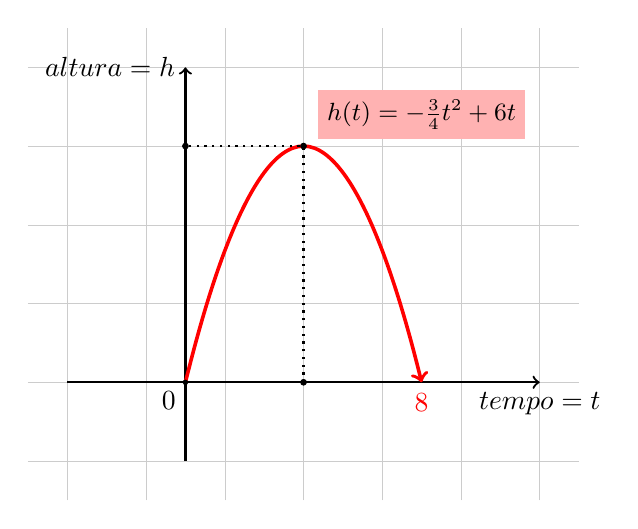
\begin{tikzpicture}

  \coordinate (a) at (-1.5,-1);
  \coordinate (b) at ($(a) + (1.5,3)$);  %($(b) + (-1.5,-1)$)
  \coordinate (bx) at ($(a) + (0,3)$);  %($(b) + (-1.5,-1)$)
  \coordinate (by) at ($(a) + (1.5,0)$);  %($(b) + (-1.5,-1)$)

  \draw[help lines,black!20] (-3.5,-2.5) grid (3.5,3.5);
  \draw[thick,->] (-3,-1) -- (3,-1) node[below] {$tempo=t$};
  \draw[thick,->] (-1.5,-2) -- (-1.5,3)   node[left]  {$altura=h$};
  \draw[line width=1.3pt,red,->] (-1.5,-1) parabola bend (0,2) (1.5,-1) node[below] {8};
  \fill (a) circle (1pt) node[below left] {$0$};
  \draw[thick, dotted] (by) -- (b) -- (bx);
  \draw[fill] (b) circle (1pt);
  \draw[fill] (by) circle (1pt);
  \draw[fill] (bx) circle (1pt);
  \node[fill=red!30] at (1.5,2.4) {\small $h(t) = - \frac{3}{4} t^2 + 6t$};
\end{tikzpicture}



\end{document}